\tikzset{every picture/.style={line width=0.75pt}} %set default line width to 0.75pt        

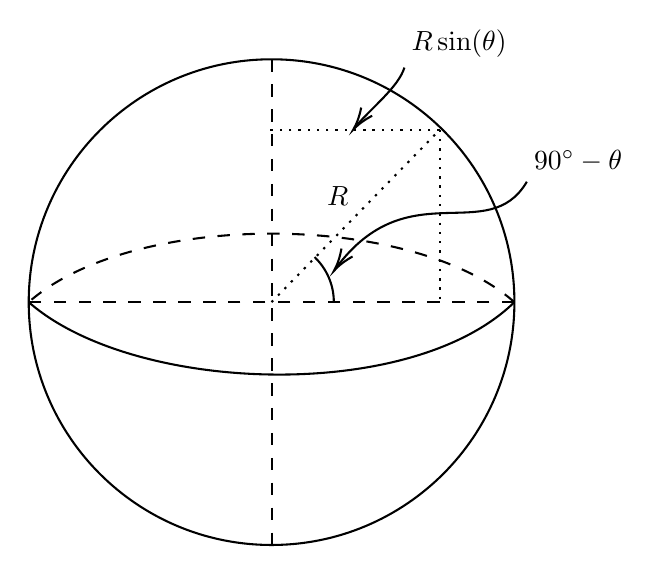
\begin{tikzpicture}[x=0.75pt,y=0.75pt,yscale=-1,xscale=1]
%uncomment if require: \path (0,485); %set diagram left start at 0, and has height of 485

%Shape: Circle [id:dp4936381296702055] 
\draw   (179,157) .. controls (179,92.38) and (231.38,40) .. (296,40) .. controls (360.62,40) and (413,92.38) .. (413,157) .. controls (413,221.62) and (360.62,274) .. (296,274) .. controls (231.38,274) and (179,221.62) .. (179,157) -- cycle ;
%Curve Lines [id:da7684497988482555] 
\draw    (179,157) .. controls (229,201) and (363,206) .. (413,157) ;
%Curve Lines [id:da031906274558686665] 
\draw  [dash pattern={on 4.5pt off 4.5pt}]  (413,157) .. controls (363,113) and (229,113) .. (179,157) ;
%Straight Lines [id:da7237618188990222] 
\draw  [dash pattern={on 4.5pt off 4.5pt}]  (296,40) -- (296,274) ;
%Straight Lines [id:da6805862140011472] 
\draw  [dash pattern={on 4.5pt off 4.5pt}]  (413,157) -- (179,157) ;
%Straight Lines [id:da6636715436204372] 
\draw  [dash pattern={on 0.84pt off 2.51pt}]  (296,157) -- (377,74) ;
%Shape: Arc [id:dp03958996945390081] 
\draw  [draw opacity=0] (316.72,135.3) .. controls (322.44,140.76) and (326,148.47) .. (326,157) -- (296,157) -- cycle ; \draw   (316.72,135.3) .. controls (322.44,140.76) and (326,148.47) .. (326,157) ;  
%Curve Lines [id:da7315028520131872] 
\draw    (419,99) .. controls (400.19,130.68) and (361.78,93.75) .. (327.05,140.56) ;
\draw [shift={(326,142)}, rotate = 305.54] [color={rgb, 255:red, 0; green, 0; blue, 0 }  ][line width=0.75]    (10.93,-3.29) .. controls (6.95,-1.4) and (3.31,-0.3) .. (0,0) .. controls (3.31,0.3) and (6.95,1.4) .. (10.93,3.29)   ;
%Straight Lines [id:da960505724523711] 
\draw  [dash pattern={on 0.84pt off 2.51pt}]  (377,74) -- (377,157.42) ;
%Straight Lines [id:da7630353719230638] 
\draw  [dash pattern={on 0.84pt off 2.51pt}]  (377,74) -- (293.58,74) ;
%Curve Lines [id:da15200728730904722] 
\draw    (360,44) .. controls (357.17,53.45) and (343.61,63.79) .. (336.47,72.5) ;
\draw [shift={(335.29,74)}, rotate = 306.71] [color={rgb, 255:red, 0; green, 0; blue, 0 }  ][line width=0.75]    (10.93,-3.29) .. controls (6.95,-1.4) and (3.31,-0.3) .. (0,0) .. controls (3.31,0.3) and (6.95,1.4) .. (10.93,3.29)   ;

% Text Node
\draw (421,95.6) node [anchor=south west] [inner sep=0.75pt]    {$90^{\circ } -\theta $};
% Text Node
\draw (334.5,112.1) node [anchor=south east] [inner sep=0.75pt]    {$R$};
% Text Node
\draw (362,40.6) node [anchor=south west] [inner sep=0.75pt]    {$R\sin( \theta )$};


\end{tikzpicture}
